\documentclass[12pt,a4paper]{article}
\usepackage{cmap}
\usepackage{mathtext}
\usepackage[T2A]{fontenc}
\usepackage{pgfplots}
\usepackage[utf8]{inputenc}
\usepackage[english,russian]{babel}  
\usepackage[export]{adjustbox}
\usepackage{amsmath}
\usepackage{amsfonts}
\usepackage{amssymb}
\usepackage[T1, T2A]{fontenc}
\usepackage{graphicx}
\usepackage[left=2cm,right=2cm,top=2cm,bottom=2cm]{geometry}
\usepackage{calc}
\usepackage{wrapfig}
\usepackage{setspace}
\usepackage{indentfirst}
\usepackage[unicode, pdftex]{hyperref}
\usepackage{subfigure}
\usepackage{booktabs}
\DeclareMathOperator{\Div}{div}
\DeclareMathOperator{\Rot}{rot}
\DeclareMathOperator{\Grad}{grad}
\usepackage[version=3]{mhchem}
\usepackage{fancyhdr}
\pagestyle{fancy}
	\fancyhead[C] {Отчёт о выполнении лабораторной работы}

\renewcommand{\footrulewidth}{ .0em }
\fancyfoot[C]{\texttt{\textemdash~\thepage~\textemdash}}

\newcommand{\parspace}{\hspace*{\parindent}}
\newcommand{\dif}{\mathrm{d}}
\usepackage{tabularx}
\usepackage{physics}
\usepackage{multirow}
\begin{document}
\begin{titlepage}
\begin{center}
    {\large МОСКОВСКИЙ ФИЗИКО-ТЕХНИЧЕСКИЙ ИНСТИТУТ (НАЦИОНАЛЬНЫЙ ИССЛЕДОВАТЕЛЬСКИЙ УНИВЕРСИТЕТ)}
\end{center}
\vspace{5.5cm}
{\huge
\begin{center}
    {\bf Лабораторная работа № 5:\\
    Определение числа Рейнольдса перехода к турбулентности в пограничном слое}
\end{center}
}
\vspace{7cm}
\begin{flushright}
{\large{ Выполнили: \\ \textbf{Рогозин Владимир \\
                        Герасимов Илья \\ 
                        Кравец Кирилл  \\
                        Казусев Степан \\
                        Дюгаева Юлия \\
                        Мисимович Милица \\
                        }
                    }
                }
                        
\end{flushright}
\vspace{1 cm}
\begin{center}
    Долгопрудный 2023
\end{center}
\end{titlepage}
\subsubsection*{Цель работы:}
Исследовать переход ламинарного режима течения в пограничном слое в турбулентный. Найти критическое значение числа Рейнольдса.

\subsection*{Введение:}
\par Проблема перехода к турбулентности в пограничном слое на протяжении уже нескольких десятилетий вызывает большой интерес исследователей.  Это обусловлено, во-первых, необходимостью решения практических задач. Во-вторых, изучение процесса возникновения турбулентности является составной частью более общей фундаментальной проблемы описания турбулентности. 
\par Переход от ламинарного течения к турбулентному в пограничном слое представляет собой сложный процесс эволюции и трансформации возмущений различной природы и их взаимодействия между собой. В соответствии с этим термин "переход к турбулентности" понимают в широком смысле как совокупность всех явлений, ответственных за разрушение ламинарного режима течения, образование турбулентного режима течения. 
\par В гидродинамике принято представлять мгновенное значение скорости в виде суммы ее среднего по времени значения и мгновенного отклонения от этой величины, которое называют пульсацией скорости. Для трех компонент скорости можно записать:
\begin{align*}
    u &= U + u', & \upsilon &= V + \upsilon', & \omega &= W + \omega'.
\end{align*}
Мерой интенсивности возмущений потока служит величина
\begin{equation*}
    \varepsilon_0 = \frac{\sqrt{(<u'^2> + <\upsilon'^2> + <\omega'^2>)/3}}{U}
\end{equation*}
(угловые скобки означают осреднение по времени; для плоскопараллельных течений W = V = 0).
\par В случае, когда возмущения во внешнем потоке изотропны, т.е. $<u'^2> = <\upsilon'^2> ~= ~<\omega'^2>$, уровень возмущений потока определяется величиной
\begin{equation*}
    \varepsilon_0 = \frac{\sqrt{<u'^2>}}{U}.
\end{equation*}
\par Процесс перехода течения в пограничном слое от ламинарного режима к турбулентному при малой интенсивности внешних возмущений состоит из трех условно разделяемых этапов: 1) генерации волн в пограничном слое, 2) их усиления по законам линейной теории и 3) нелинейного разрушения ламинарного режима течения.Описанная последовательность стадий перехода схематически показана на рис.~\ref{1}
\newpage
\begin{figure}[h!]
    \centering
    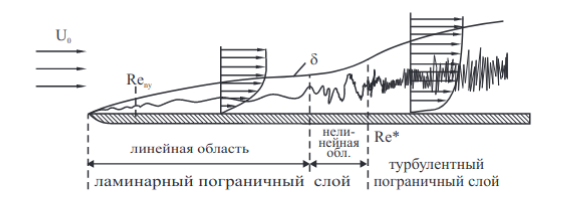
\includegraphics[width = 0.8 \textwidth]{lam_to_turbo.png}
    \caption{Основные стадии перехода к турбулентности в пограничном слое}
    \label{1}
\end{figure}
\subsection*{Обоснование методики эксперимента}
\par Переход течений в пограничном слое в трубе и на пластине из ламинарной формы в турбулентную заметнее всего отражается на распределении скоростей в пограничном слое и скорости нарастания толщины пограничного слоя. Этот факт хорошо иллюстрирует рис.\ref{pic2}
\begin{wrapfigure}{l}{0.3\linewidth}
	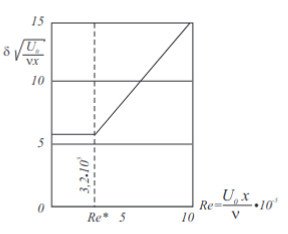
\includegraphics[width=1 \linewidth]{2.png}
	\caption{Зависимость безразмерной толщины пограничного слоя от числа Рейнольдса}
	\label{pic2}
\end{wrapfigure}
Условия проведения этого эксперимента были таковы, что после достижения числом Рейнольдса значения $Re_{кр} = U_0x/\nu > 3.2 \cdot 10^5$ толщина пограничного слоя начинала сильно нарастать. В месте с переходом от ламинарного движения к турбулентному наблюдается и резкое изменение распределения скоростей в пограничном слое. Уменьшение степени турбулентности приводит к смещению вниз по потоку области перехода от ламинарноготечения к турбулентному в пограничном слое, т.е. к увеличению $Re_{кр}$.
\begin{wrapfigure}{r}{0.4\linewidth}
	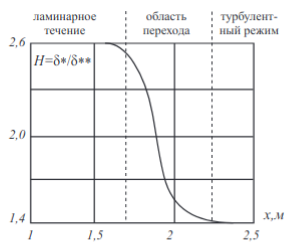
\includegraphics[width=1 \linewidth]{3.png}
	\caption{Изменение формпараметра H = $\delta^*/\delta^{**}$ для пограничного слоя на пластине в области перехода}
	\label{pic3}
\end{wrapfigure}
С изменением распределения скоростей в области перехода связано уменьше-
ние формпараметра H = $\delta^*/\delta^{**}$, приведенное на рис. \ref{pic3}, где $\delta^*$ -- толщина вытеснения, $\delta^{**}$ -- толщина потери импульса. В пограничном слое на пластине формпараметр уменьшается от значения Н = 2.6, в ламинарной области -- до значения Н = 1.4, в турбулентной области.
\par Изменение распределения скорости в пограничном слое при переходе из ламинарной формы движения в турбулентную можно использовать для простого способа определения положения точки перехода (точнее говоря, области перехода). Принцип такого определения пояснен на рис.\ref{pic4}
\begin{figure}[h!]
    \centering
    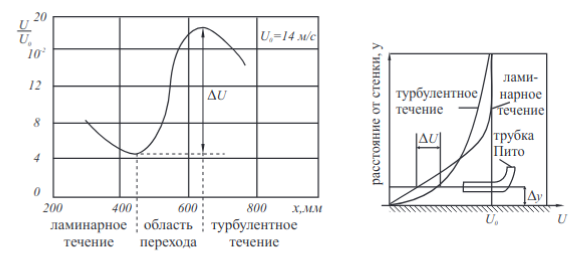
\includegraphics[width = 1.0 \textwidth]{4.png}
    \caption{К определению положения точки перехода ламинарного режима в турбулентный в пограничном слое при $U_o= const, x = var$}
    \label{pic4}
\end{figure}

\par Изменение скорости нарастания толщины пограничного слоя (зависимости $\delta$(x)) при изменении режима течения может быть использовано для определения числа Рейнольдса перехода к турбулентности, построенного по скорости внешнего потока и расстоянию, нa котором нарастает пограничный слой. Трубка полного напора в этом случае должна устанавливаться во внешней части пограничного слоя. Если при заданной скорости пограничный слой перед трубкой полного напора ламинарный, тo увеличением скорости можно добиться, чтобы переход к турбулентности происходил перед трубкой полного напора. Отношение скорости в месте установки трубки полного напора в пограничном слое U к скорости внешнего потока U0 в зависимости от скорости внешнего потока будет в этом случае иметь характер, приведенный на рис. \ref{pic5}. При ламинарном режиме течения в пограничном слое перед трубкой полного напора увеличение скорости приведет к уменьшению толщины пограничного слоя и увеличению отношения $U/U_0$. Когда переход будет происходить непосредственно перед трубкой полного напора, увеличение скорости приведет к тому, что трубка будет все глубже погружаться в быстронарастающий по координате x турбулентный пограничный слой (рис. \ref{pic5}), а это, в свою очередь приведет к уменьшению $U/U_0$.
\begin{figure}[h!]
    \centering
    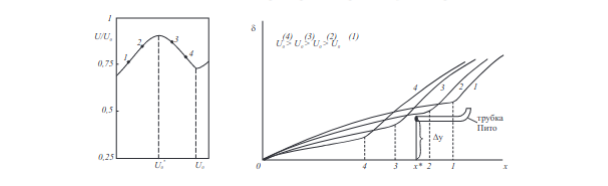
\includegraphics[width = 1.0 \textwidth]{5.png}
    \caption{К определению положения точки перехода ламинарного режима в турбулентный в пограничном слое при $U_0= const, x = var$}
    \label{pic5}
\end{figure}

\newpage
\subsection*{Экспериментальная установка}
Основными узлами экспериментальной установки являются: система подачи рабочего газа (воздуха), устройство для формирования пограничного слоя и система измерений. Основным элементом узла, формирующего пограничный слой, является аэродинамическая дозвуковая труба 1 с набором цилиндрических насадков 4 различной длины, называемых рабочими каналами, закрепленная на станине 8 (рис. \ref{pic6}). Для выравнивания потока и подавления турбулентных пульсаций внутри трубы установлена система латунных сеток 2. Аэродинамическая труба создает на выходе конфузора 3 равномерный поток воздуха с низким уровнем турбулентных пульсаций (менее 0.5$\%$) в необходимом диапазоне скоростей (7–15 м/сек). Выходящий из конфузора поток воздуха попадает в цилиндрический рабочий канал 4 диаметром 49 мм, на внутренней поверхности которого нарастает пограничный слой. Толщина этого пограничного слоя мала по сравнение с радиусом трубы, поэтому все его параметры (профиль скорости, толщина, формпараметр и т.д.) близки к соответствующим характеристикам пограничного слоя на плоской пластине. Измерения проводятся на срезе рабочего канала. Система измерения состоит из двух наклонных, либо U -образных манометров 7, соединенных с трубками полного напора 5, закрепленных на координатнике 6, обеспечивающим их перемещениев диаметральном направлении в плоскости среза рабочего канала.
\begin{figure}[h!]
    \centering
    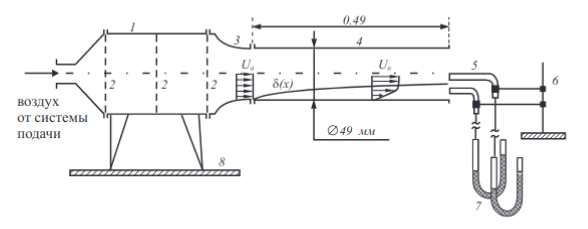
\includegraphics[width = 1.0 \textwidth]{6.png}
    \caption{Cхема установки и система измерений}
    \label{pic6}
\end{figure}

\subsection*{Теоретические сведения}
    Для сжимаемого идеального газа в адиабатическом процессе можно записать:
    \begin{equation*}
        \frac{p}{p_0} = \left(1 + \frac{\gamma - 1}{2} M^2\right)^{- \frac{\gamma}{\gamma - 1}}
    \end{equation*}
     где p - давление в потоке, $p_0$ - атмосферное давление, M - число Маха.
    \par Учтем малость числа Маха:
    \begin{equation}\label{eq:1}
        p_0 = p + \frac{\rho u^2}{2}
    \end{equation}
    \par В практических расчетах коэффициент динамической вязкости можно рассчитать:
    \begin{equation}\label{eq:2}
        \mu = \mu_0 \cdot \left(\frac{T}{273}\right)^{3/4},
    \end{equation}
    где $\mu_0 = 1.75\cdot 10^{-5} Па \cdot c$ \\
    Число Рейнольдса вычисляется по формуле:
    \begin{equation}\label{eq:3}
        Re = \frac{\rho u L}{\mu}
    \end{equation}
    Для пограничного слоя характерен следующий профиль скорости:\\
    \begin{figure}[h!]
        \centering
        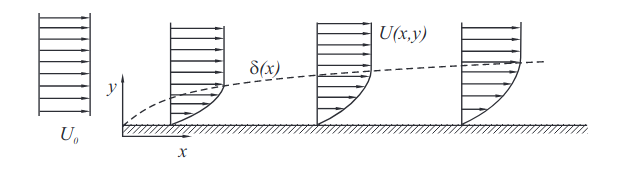
\includegraphics[width = 1.0 \textwidth]{last.png}
        \caption{Пограничный слой}
        \label{fig:my_label}
    \end{figure}
    Толщину пограничного слоя можно оценить:
    \begin{enumerate}
        \item Для турбулентного потока
        \begin{equation}
            \delta_{\text{турб}}= 0.37 \cdot x \left(\frac{U_0 x}{\nu}\right)^{-1/5} \sim \frac{1}{Re_{\text{турб}}}^{1/5}
        \end{equation}\label{eq:4}
        \item Для ламинарного потока
        \begin{equation}
            \delta_{\text{лам}} = 5\cdot x \left(\frac{U_0x}{\nu}\right)^{-1/2} \sim \frac{1}{Re_{\text{лам}}}^{1/2}
        \end{equation}\label{eq:5}
    \end{enumerate}
    
\subsection*{Ход работы}
    \subsubsection*{Начальные условия}
    \begin{enumerate}
        \item $T_0$ = 295 K
        \item $p_{\text{атм}}$ = $10^{5}$ Па
        \item $R_{\text{атм}}$ = 286.7 $\frac{\text{дж}}{\text{кг}\cdot \text{К}}$
        \item $\mu_{\text{атм}}$ = $1.85 \cdot 10^{-5} \text{Па} \cdot с$
        \item L = 0.49 м
        \item $\rho_{\text{атм}}$ = 1.19 кг/$\text{м}^3$
    \end{enumerate}
    \begin{enumerate}
        
    
    \item \par Из формулы (\ref{eq:1}), для скорости ядра получили:
    \begin{equation*}
        u = \sqrt{\frac{2\Delta p}{\rho_{атм}}} = K_1 \sqrt{\Delta p},
    \end{equation*}
    где $K_1 = 1.30$ м$^{3/2}$/кг$^{1/2}$
    \item \par Из формулы (\ref{eq:3}) для числа Рейнольда получили:
    \begin{equation*}
        Re_L = K_2 \sqrt{\Delta p},
    \end{equation*}
    где $K_2 = 4 \cdot 10^4 $ Па $^{-1/2}$

    \item Получили экспериментальные значения:
    \begin{table}[h!]
        \centering
        \begin{tabular}{|c|c|c|c|c|c|c|c|}
        \hline
    V &   $\Delta P_{b}$ Па&    $\Delta P_{c}, КПа$ &  $U/U_c $& $U_c$ м/с& $Re_L$ & $\left(P_{b}/P_{c}\right)^{2}$ &  $P_{b}/P_{c}$ \\
    \hline
      80 &  22 &   39 &  0.75 &   8.12 &  249799 &  0.32 &  0.56 \\ \hline
      90 &  31 &   46 &  0.82 &   8.82 &  271293 &  0.45 &  0.67 \\ \hline
      100 &  43 &   55 &  0.88 &   9.64 &  296647 &  0.61 &  0.78 \\ \hline
      110 &  50 &   63 &  0.89 &  10.32 &  317490 &  0.63 &  0.79 \\ \hline
      120 &  53 &   71 &  0.86 &  10.95 &  337045 &  0.56 &  0.75 \\ \hline
      130 &  54 &   79 &  0.83 &  11.55 &  355527 &  0.47 &  0.68 \\ \hline
      140 &  56 &   87 &  0.80 &  12.13 &  373095 &  0.41 &  0.64 \\ \hline
      150 &  59 &   96 &  0.78 &  12.74 &  391918 &  0.38 &  0.61 \\ \hline
      160 &  63 &  104 &  0.78 &  13.26 &  407921 &  0.37 &  0.61 \\ \hline
      180 &  71 &  120 &  0.77 &  14.24 &  438178 &  0.35 &  0.59 \\ \hline
      200 &  80 &  135 &  0.77 &  15.10 &  464758 &  0.35 &  0.59 \\ \hline
      220 &  88 &  150 &  0.77 &  15.92 &  489897 &  0.34 &  0.59 \\ \hline
      240 &  98 &  166 &  0.77 &  16.75 &  515363 &  0.35 &  0.59 \\ \hline
        \end{tabular}
        \caption{}
        \label{tab:1}
    \end{table}
    
    \begin{figure}[h!]
        \centering
        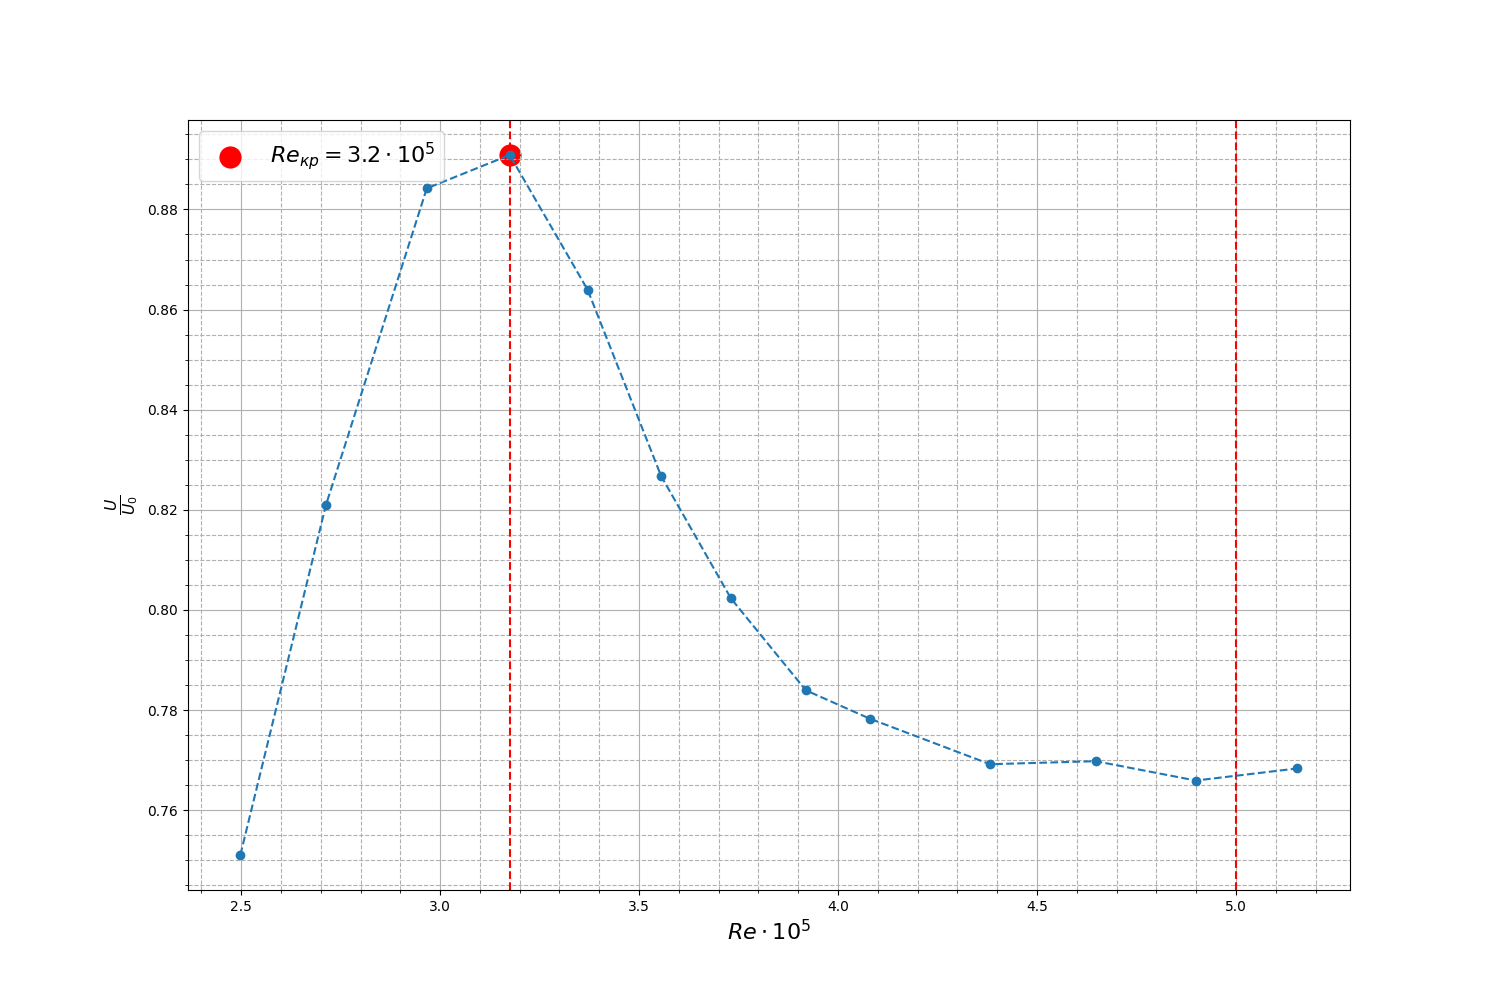
\includegraphics[width = 1 \textwidth]{plot3_3.png}
        \caption{}
        \label{fig:1}
    \end{figure}
    \item Определили $Re_{\text{кр}} = 3.2 \cdot 10^5$ при котором будет переход от ламинарного к турбулентному потоку.
    \item Из полученных данных(\ref{tab:1}, \ref{fig:1}) видно, что при V = 105 В будет явный ламинарный поток, а при V = 230 В будет наблюдаться турбулентный поток.
    \item Исследовали потоки при 105В и 230В, перемешая трубку Пито от пристеночного потока к центральному.
    
    \begin{table}[h!]
        \centering
        \begin{tabular}{|c|c|c|c|c|}
        \hline
          y, мм &   $\Delta P$, КПа & U, м/с & U/$U_c$ & $Re_L$ \\ \hline
        0.25 &   3 &  2.25 &  0.23 &   69282 \\ \hline
        0.50 &   8 &  3.68 &  0.37 &  113137 \\ \hline
        0.75 &  13 &  4.69 &  0.48 &  144222 \\ \hline
        1.00 &  20 &  5.81 &  0.59 &  178885 \\ \hline
        1.50 &  34 &  7.58 &  0.77 &  233238 \\ \hline
        2.00 &  43 &  8.52 &  0.87 &  262297 \\ \hline
        2.50 &  49 &  9.10 &  0.93 &  280000 \\ \hline
        3.25 &  54 &  9.55 &  0.98 &  293938 \\ \hline
        4.00 &  55 &  9.64 &  0.99 &  296647 \\ \hline
        5.00 &  56 &  9.73 &  1.00 &  299332 \\ \hline 
        6.00 &  56 &  9.73 &  1.00 &  299332 \\ \hline
        7.00 &  56 &  9.73 &  1.00 &  299332 \\ \hline
        \end{tabular}
        \caption{Ламинарный поток V = 105B, $Re_L$ $\sim$ 3.1$\cdot 10^{5}$}
        \label{tab:2}
    \end{table}

    \begin{table}[h!]
        \centering
        \begin{tabular}{|c|c|c|c|c|}
        \hline
          y, мм &   $\Delta P$, КПа & U, м/с & U/$U_c$ & $Re_L$ \\ \hline
        0.25 &    3 &   2.25 &  0.14 &   69282 \\ \hline
        0.50 &   23 &   6.23 &  0.38 &  191833 \\ \hline
        0.75 &   47 &   8.91 &  0.55 &  274226 \\ \hline
        1.00 &   64 &  10.40 &  0.64 &  320000 \\ \hline
        1.50 &   75 &  11.26 &  0.69 &  346410 \\ \hline
        2.00 &   83 &  11.84 &  0.73 &  364417 \\ \hline
        2.50 &   89 &  12.26 &  0.76 &  377359 \\ \hline
        3.25 &   99 &  12.93 &  0.80 &  397994 \\ \hline
        4.00 &  110 &  13.63 &  0.84 &  419523 \\ \hline 
        5.00 &  120 &  14.24 &  0.88 &  438178 \\ \hline
        6.00 &  130 &  14.82 &  0.91 &  456070 \\ \hline
        7.00 &  139 &  15.33 &  0.95 &  471593 \\ \hline
        8.50 &  150 &  15.92 &  0.98 &  489897 \\ \hline
        10.00 &  154 &  16.13 &  0.99 &  496386 \\ \hline
        11.50 &  155 &  16.18 &  1.00 &  497995 \\ \hline 
        13.00 &  155 &  16.18 &  1.00 &  497995 \\ \hline
        \end{tabular}
        \caption{Турбулентный поток V = 230B, $Re_L$ $\sim 5 \cdot 10^{5}$}
        \label{tab:3}
    \end{table}
    \newpage
    \item Построили график:
    \begin{figure}[h!]
        \centering
        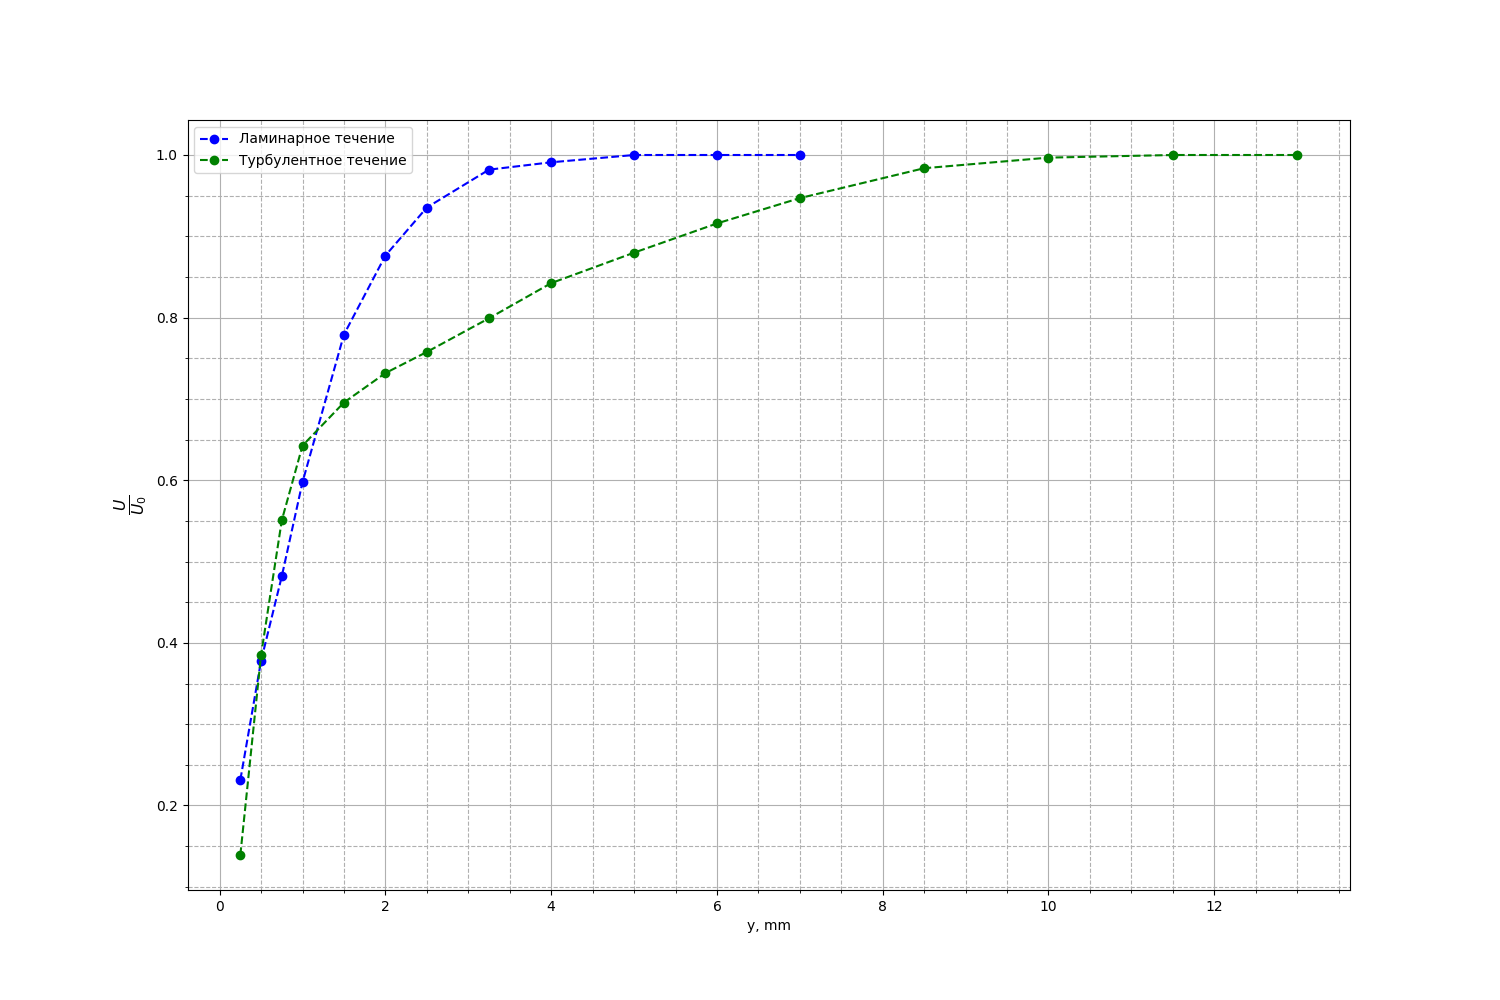
\includegraphics[width = 1 \textwidth]{plot_1.png}
        \caption{}
        \label{fig:3}
    \end{figure}
    \item Оценили толщину пограничных слоев по формулам(\ref{eq:4}, \ref{eq:5}):
    \begin{align*}
        \delta_{\text{лам}} &\sim  1.8 \cdot 10^{-3} & \delta_{\text{турб}} &\sim 0.0725 \\
    \end{align*}
    \end{enumerate}
    \subsection*{Вывод}
    \begin{enumerate}
        \item Исследовали профиль скоростей в пограничном слое. В турбулентном режиме течения характерная толщина в пограничного слоя больше, в связи с большим трением в этой области.
        \item Определили критическое значения числа Рейнольдса $Re_L = 3.2 \cdot 10^5$ перехода из ламинарного режима в турбулентный.
        \item Из графика (\ref{fig:3}) можно сделать вывод, что поле течения можно разбить на область пограничного слоя, в котором действуют силы трения и область, в которой этими силами можно пренебречь и использовать теорию идеальной жидкости. 
    \end{enumerate}
\end{document}
